
%(BEGIN_QUESTION)
% Copyright 2006, Tony R. Kuphaldt, released under the Creative Commons Attribution License (v 1.0)
% This means you may do almost anything with this work of mine, so long as you give me proper credit

Her vises mekanismen for en forenklet (uten forsterkerrelé, uten biasfjær) pneumatisk kun-proporsjonal regulator:

$$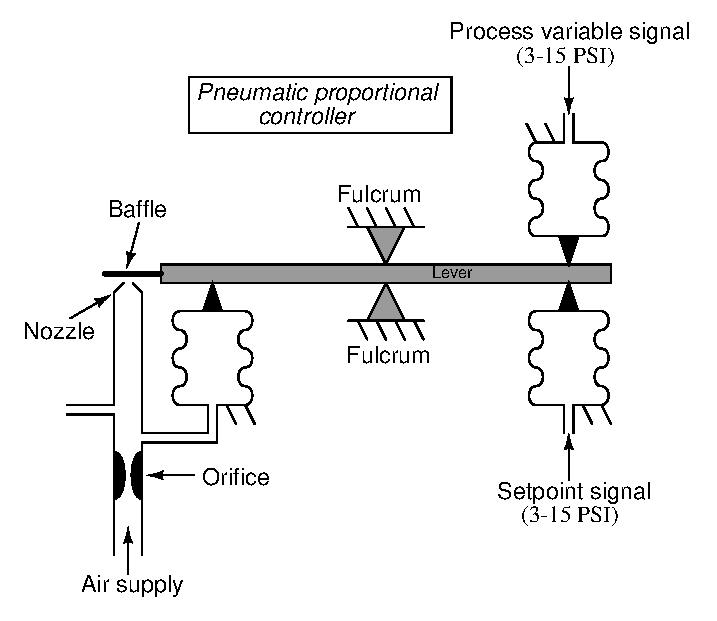
\includegraphics[width=15.5cm]{i01542x01.eps}$$

Forklar hvordan denne regulatormekanismen fungerer, og sørg for å inkludere begrepet {\it negativ tilbakekobling} i forklaringen.

\vskip 10pt

\filbreak

Anta at denne pneumatiske regulatoren får et problem: det korte røret som kobler til tilbakekoblingsbelgen blir helt tett. Dette gjør at tilbakekoblingsbelgen ikke kan registrere lufttrykket ved dysen:

$$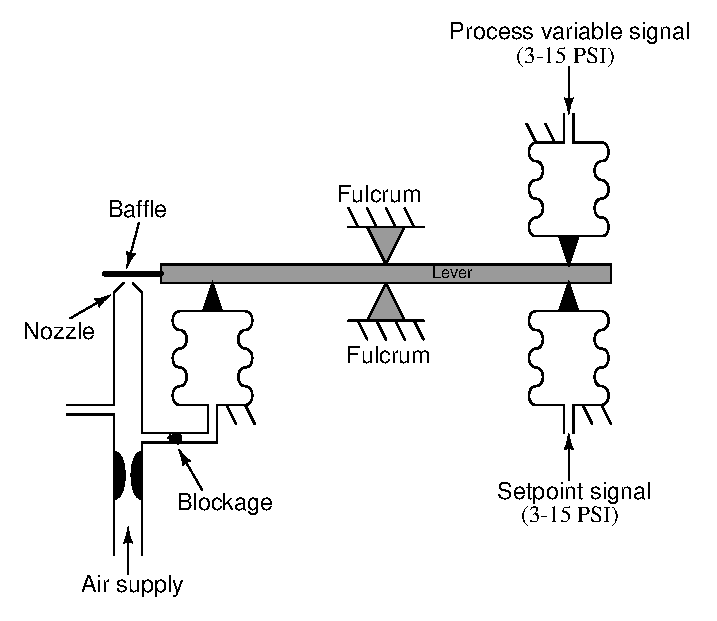
\includegraphics[width=15.5cm]{i01542x02.eps}$$

Beskriv og forklar hvilken effekt denne rørblokkeringen vil ha på regulatorens oppførsel.

\vskip 10pt

\filbreak

Anta nå at det samme røret bare er {\it delvis} tett, slik at luftpassasjen gjennom røret går saktere og belgtrykket kommer tidsmessig etter dysetrykket:

$$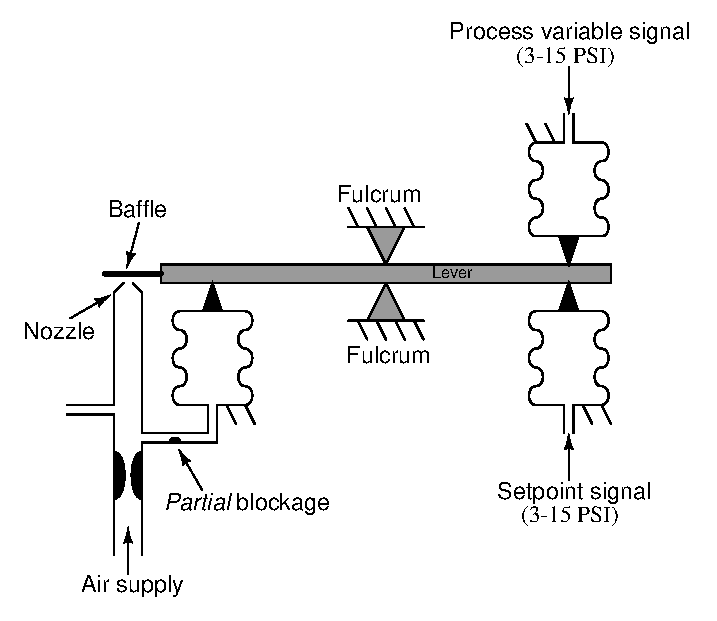
\includegraphics[width=15.5cm]{i01542x04.eps}$$

\underbar{file i01542}
%(END_QUESTION)





%(BEGIN_ANSWER)

Jeg svarer på spørsmålet om total rørblokkering med et motspørsmål: hva vil skje i følgende operasjonsforsterkerkrets hvis tilbakekoblingsmotstanden blir brutt (åpen krets)?

$$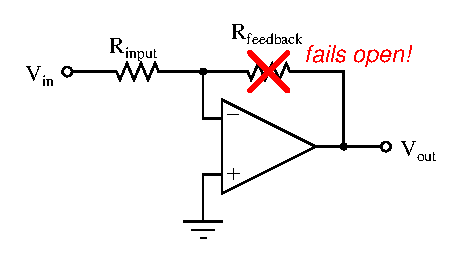
\includegraphics[width=15.5cm]{i01542x03.eps}$$

Ved delvis blokkering vil regulatoren ``overreagere'' på raske endringer i enten PV eller SP, og deretter falle til ro på den normale utgangssignalverdien som forventes av en proporsjonal regulator.

%(END_ANSWER)





%(BEGIN_NOTES)



%INDEX% Control, proportional: pneumatic force-balance controller

%(END_NOTES)

